% -------------------------------------------------------------------------------------------------
% ------------------------------------------ METHODS --------------------------------------------
% -------------------------------------------------------------------------------------------------

\chapter{Methods}
\label{Methods}

\pagestyle{fancy}

\raggedbottom

\fancypagestyle{plain}{
\fancyhf{} 
\fancyfoot[RO, LE]{\thepage} 
\renewcommand{\headrulewidth}{0pt}}

\fancyhf{}
\fancyhead[RO, LE]{Methods}
\fancyfoot[RO,LE]{\thepage}

\section{Construction of the dataset}
Three dimensional structures for protein dimers were retrieved from Protein Data Bank \citep{Berman2000}. The search for proteins with 2 chains (Asymmetrical Unit) returned 32871 structures. In order to remove redundancy, the above dataset was culled using the PISCES web server \citep{Wang2005} with the parameters given in Table \ref{PISCES_table}. This resulted in a non-redundant dataset comprising of 6870 structures. Further filtering based on Buried Surface Area (BSA) was done.  Buried Surface Area is defined as:
\begin{equation}
BSA =  \sum\limits_{n = 1}^{N_{subunits}} ASA_{\;free}^{\;S_{n}} - ASA_{\;Complex}
\end{equation}
where, $ASA_{\;free}^{\;S_{n}}$, is the solvent accessible surface area of the unbound subunits of the protein complex and $ASA_{\;Complex}$ is the solvent accessible surface area for the bound complex. BSA for the dimers was computed as per Eq. 2.1 using MODELLER \citep{Sali1993} and structures satisfying $400 \; \si{\angstrom}^2 \leq BSA \leq 2500 \; \si{\angstrom}^2$ were taken to construct the final dataset. The lower bound on the BSA was put to remove false positives from crystal contact artifacts whereas the upper limit excluded structures with intertwined subunits. The final dataset comprising of 4060 protein dimers was divided into two sets: a training set of 3764 dimers, which were used for constructing the potential and a testing set of 296 dimers, used for benchmarking the statistical potentials. In order to make accurate predictions using statistical potentials, the number of samples in the training set should be large while keeping a reasonable number of samples in the testing set. Hence the division of the dimer set was made such that the testing set is $\sim$ 10 \% of the training set. The PDB codes of the structures comprising the training and the testing set are listed in Appendix 1.

\begin{center}
	\begin{tabular}{ | l | l | }
	\hline
	Sequence Percentage Identity & <= 40 \% \\ \hline
	Resolution & 0.0 $\thicksim$ 3.0 \\ \hline
	R-Factor & 0.3 \\ \hline
	Sequence Length & 40 $\thicksim$ 10000 \\ \hline
	Non X-ray entries & Excluded \\ \hline
	CA-only entries & Excluded \\ \hline
	Cull PDB by & Entry \\ \hline
	Cull chains within entries & No \\ \hline
	\end{tabular}
	\captionof{table}{Parameters used for removing redundancy of the PDB dataset}
	\label{PISCES_table}
\end{center}

\section{Construction of Statistical Potentials}
A series of Statistical Potentials were constructed using the protein dimers from the training dataset constructed above. Inter-atomic distances at different thresholds were computed for each structure using the 'cell list' implementation (borrowed from Neelesh Soni). Two amino acid residues were defined as interacting if any relevant atom of residue $A$ of type $i$ was within the distance threshold of any relevant atom of residue $B$ of type $j$. Residue $A$ and Residue $B$ belong to different subunits of the protein complex. 96 different potentials were built using different values for five parameters : the contacting atom types (main chain-main chain, main chain-side chain, side chain-side chain or all), the weighing scheme for assigning weights to distinct residue interactions (cifa potential vs ipa potential),  nature of the weights (derived at a single distance (norm) vs averaged over multiple distance (cmpd)), weights in the reference state (avg vs no\_avg) and the distance threshold for contact participation (4, 6, or 8 {\AA}). The combination of the different values for these five parameters gave rise to $4 \times 2 \times 2 \times 2 \times 3 \;=\;96$ different potentials.

\subsection{Two-Body Potentials}

\subsubsection{The cifa potential} 
\vspace{24pt}
\begingroup
\large
\begin{equation}
\mathrm{S}_{i,j} = -\log \left[ \left(\sum\limits_{\forall \;\mathrm{interfaces}} \dfrac{\dfrac{ f_{\;ij}^{\;int}}{\sum\limits_{\forall ab}{cifa}_{\;ab}^{\;int}} \times \dfrac{{cifa}_{\;ij}^{\;int}}{\mathrm{max}({cifa}_{\;ij}^{\;int})}}{\dfrac{f_i}{N_m}\dfrac{f_j}{N_n} \times \langle {cifa}_{\;ij}^{\;int} \rangle} \right) \div N_{total} \right] 
\end{equation}
\endgroup

\begingroup
\setlength\abovedisplayskip{0pt}
\begin{eqnarray}
\mathrm{where,} \nonumber \\
f_{ij}^{int} &=& \mathrm{frequency\;of}\;i-j\; \mathrm{residue\;pairs\;across\;the\;interface}
\nonumber \\
{cifa}_{ij}^{int} &=& \mathrm{min}\left[ \frac{\mathrm{interacting \; atoms}_{\;i}}{\mathrm{total \; atoms}_{\;i}}, \frac{\mathrm{interacting \; atoms}_{\;j}}{\mathrm{total \; atoms}_{\;j}}\right]
\nonumber \\
cifa_{\;ab}^{\;int} &=& \mathrm{frequency\;of\;any\;residue\;pair}\;a-b\; \mathrm{weighted\;by\;their\;respective\;}cifa
\nonumber \\
\dfrac{f_i}{N_m} &=& \mathrm{frequency\;of\;residues\;of\;type\;}i \mathrm{\;in\;the\;subunit\;}m
\nonumber \\
\dfrac{f_j}{N_n} &=& \mathrm{frequency\;of\;residues\;of\;type\;}j \mathrm{\;in\;the\;subunit\;}n
\nonumber \\
N_m, N_n &=& \mathrm{Number\;of\;subunits\;in\;subunits\;} m\; \mathrm{and\;} n\; \mathrm{respectively}
\nonumber \\
\langle {cifa}_{\;ij}^{\;int} \rangle &=& \mathrm{average\;value\;of}\;cifa\;\mathrm{observed\;in\;the\;dataset\;for}\;i-j\; \mathrm{pairs\;across\;the\;interface}
\nonumber \\
N_{total} &=& \mathrm{total\;number\;of\;protein\;complexes\;in\;the\;dataset} \nonumber
\end{eqnarray}
\endgroup

The observed probability for residue pairs of type $i$ and $j$ that belonged to different subunits and occurred within a distance threshold in a protein complex was weighted by $cifa$, the minimum of the fraction of the total atoms in each residue that were within the distance threshold. This weight was further normalised by max ($cifa_{ij}$), the maximum $cifa$ value for the $i,j$ residue pair observed in the dataset. The probability of the occurrence of an amino acid pair of the type $i, j$ was computed based on the occurrences of the residues $i$ and $j$ in their respective subunits. This probability weighted by the average value of $cifa$ observed in the dataset for the residue pair $i, j$ forms the expected probability for a residue pair of the type $i, j$.

\vspace{24pt}

\subsubsection{The ipa potential}

\vspace{24pt}

\begingroup
\large
\begin{equation}
\mathrm{S}_{i,j} = -\log \left[ \left( \sum\limits_{\forall \; \mathrm{interfaces}} \dfrac {\dfrac{ f_{\;ij}^{\;int}}{\sum\limits_{\forall ab} \mathrm{\alpha}_{\;ab}} \times \alpha_{ij}} {\dfrac{f_i}{N_m} \dfrac{f_j}{N_n} \times \langle \alpha_{ij} \rangle} \right) \div N_{total} \right]
\end{equation}
\endgroup

\begingroup
\setlength\abovedisplayskip{0pt}
\begin{eqnarray}
\mathrm{where,} \nonumber \\
\alpha_{ij} &=& \dfrac{{ipa}_{\;ij}^{\; int}}{\mathrm{max} \; ({ipa}_{\;ij}^{\;int})} \nonumber \\
\nonumber \\
\mathrm{ipa} &=&  \mathrm{number\; of \;interacting\; pairs\; of\; atoms \; of\;residue\; types\;} i \;\mathrm{and} \; j
\nonumber \\
\alpha_{\;ab}^{\;int} &=& \mathrm{frequency\;of\;any\;residue\;pair}\;a-b\; \mathrm{weighted\;by\;their\;respective\;}\alpha
\nonumber \\
\dfrac{f_i}{N_m} &=& \mathrm{frequency\;of\;residues\;of\;type\;}i \mathrm{\;in\;the\;subunit\;}m
\nonumber \\
\dfrac{f_j}{N_n} &=& \mathrm{frequency\;of\;residues\;of\;type\;}j \mathrm{\;in\;the\;subunit\;}n
\nonumber \\
N_m, N_n &=& \mathrm{Number\;of\;subunits\;in\;subunits\;} m\; \mathrm{and\;} n\; \mathrm{respectively}
\nonumber \\
\langle {\alpha}_{\;ij}^{\;int} \rangle &=& \mathrm{average\;value\;of}\; \alpha \;\mathrm{observed\;in\;the\;dataset\;for}\;i-j\; \mathrm{pairs\;across\;the\;interface}
\nonumber \\
N_{total} &=& \mathrm{total\;number\;of\;protein\;complexes\;in\;the\;dataset} \nonumber
\end{eqnarray}
\endgroup

In the second potential, the observed probability for residue pairs of type $i$ and $j$ that occurred within a distance threshold in a protein was weighted by $ipa$, the total number of interacting pairs of atoms between two residues. Similar to the first potential, this weight was further normalised by max ($ipa_{ij}$), the maximum $ipa$ value observed for the $i,j$ residue pair in the dataset. The reference state for this potential was similar to the reference state in the $cifa$ one, with the average value of $ipa$ observed in the dataset for the residue pair $i,j$ as the weight for the expected probability.

\par
As Glycines lacks a side chain, they were handled in the following three ways in the side chain-side chain potentials. In the first scenario, assuming that all atom potential values should be representative of interactions concerning Glycine residues in the side chain-side chain case, the potential values for side chain-side chain interactions involving Glycine were borrowed from the corresponding all atom potentials. In the second scenario, following the assumption that side chain interactions are the major drivers for specificity in protein-protein interactions, the Glycine interactions were given a positive, hence unfavourable value of 1.38. For the third scenario, the potential value for all Glycine interactions was set to 0, the assumption underlying this scenario was that the occurrence of Glycine on protein-protein interfaces is random and hence the log odds of the observed probability against the expected probability of Glycine pairs is 1. The performance of the potential values for the three different scenarios were tested on the benchmark test by considering the number of native structures that were ranked the best against the randomised scores.

\vfill

\subsection{Multibody Potentials}
Pairwise statistical potentials consider a protein-protein interface to be comprised of isolated residue pairs and hence devoid of any structural context. In a bid to include the structural neighbourhood of an amino acid residue while constructing the potential, 5-body statistical potentials were constructed, following the formulation of the two-body potentials. The interface of each protein complex was decomposed into 5-body amino acid cliques based on the interatomic distances between the residues. In graph  theory, a clique is a special graph in which every vertex is connected to every other vertex in the graph. Two different distance thresholds, the intra-domain distance threshold and the inter-domain distance threshold, were used to define the connections in the clique, $(i)$ the intra-domain threshold of 5 \AA \; and $(ii)$ the inter-domain threshold of 8.5 \AA. We define two amino acids to be connected if any atom of residue $A$ lies within a distance threshold $R_0$ of any atom of residue $B$ (Fig \ref{clique}). 
For these definitions, two cases were tested, Case $(I)$ (the unweighted case), where the potentials were computed according to the formulation given in Eq. \ref{mb_eqn} and Case $(II)$ (the weighted case), where the potentials in Eq. \ref{mb_eqn} were weighted using the average pairwise cifa values (borrowed from the two-body potentials) for the residue pairs constituting the cliques.
\vspace{36pt}

\begin{figure}[hb]
	\centering
	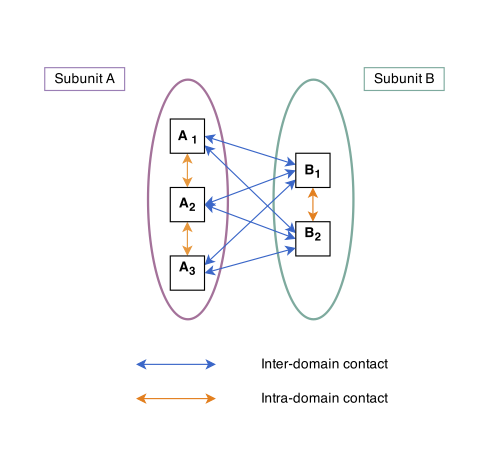
\includegraphics{./methods/clique.eps}
	\caption[Schematic representation of a 5-body clique]{Schematic representation of a 5-body clique. Residues $A_1, A_2$ and $A_3$ belong to Subunit A of the protein complex whereas Residues $B_1$ and $B_2$ belong to Subunit B of the protein complex. The contacts between residues from the same subunit are termed as intra-domain contacts (shown by orange arrows) and the contacts between residues from different subunits are termed as inter-domain contacts (depicted by the blue arrows).}
	\label{clique}
\end{figure}

\vfill

\begingroup
\large
\begin{equation}
\mathrm{S}_{A_{1}A_{2}A_{3}B_{1}B_{2}} = -\log \left[ \left( \sum\limits_{\forall\; \mathrm{interfaces}} \dfrac{\dfrac{\vphantom{\frac{a}{b}} f_{A_{1}A_{2}A_{3}B_{1}B_{2}}}{\vphantom{\frac{a}{b}}\sum\limits_{\forall \; \alpha,\beta,\gamma,\delta,\epsilon} \;(f_{\alpha\beta\gamma\delta\epsilon})}}{\dfrac{\vphantom{\frac{a}{b}}f_{A_1}^M}{\vphantom{\frac{a}{b}}\sum\limits_{x = 1}^{20} f_{x}^M}\dfrac{\vphantom{\frac{a}{b}}f_{A_2}^M}{\vphantom{\frac{a}{b}}\sum\limits_{x = 1}^{20} f_{x}^M}\dfrac{\vphantom{\frac{a}{b}}f_{A_3}^M}{\vphantom{\frac{a}{b}}\sum\limits_{x = 1}^{20} f_{x}^M}\dfrac{\vphantom{\frac{a}{b}}f_{B_1}^N}{\vphantom{\frac{a}{b}}\sum\limits_{x = 1}^{20} f_{y}^N}\dfrac{\vphantom{\frac{a}{b}}f_{B_2}^N}{\vphantom{\frac{a}{b}}\sum\limits_{x = 1}^{20} f_{y}^N}} \right) \div N_{total} \right]
\label{mb_eqn}
\end{equation}
\endgroup

\begingroup
\setlength\abovedisplayskip{0pt}
\begin{eqnarray}
\mathrm{where,} \nonumber \\
A_{1}, A_{2}, A_{3} &\mathrm{\;are}&\; \mathrm{residues\;that\;belong\;to\;subunit\;}M
\nonumber \\
B_{1}, B_{2} &\mathrm{\;are}&\; \mathrm{residues\;that\;belong\;to\;subunit\;}N
\nonumber \\
f_{A_{1}A_{2}A_{3}B_{1}B_{2}} &=& \mathrm{frequency\;of\;the\;clique\;}A_{1}A_{2}A_{3}B_{1}B_{2}\; \mathrm{across\;the\;interface}
\nonumber \\
f_{\alpha\beta\gamma\delta\epsilon} &=& \mathrm{frequency\;of\;any\;5-body\;clique\;}\alpha\beta\gamma\delta\epsilon \; \mathrm{across\;the\;interface} 
\nonumber \\
\dfrac{f_{A_{1}}^{M}}{\sum\;f_{x}^M} &=& \mathrm{frequency\;of\;the\;residues\;of\;type\;}A_{1}\; \, \mathrm{in\;the\;subunit\;}M; \; \mathrm{similarly\;for\;} \dfrac{f_{A_{3}}^{M}}{\sum\;f_{x}^M} \; \mathrm{and} \; \dfrac{f_{A_{3}}^{M}}{\sum\;f_{x}^M}
\nonumber \\
\dfrac{f_{B_{1}}^{M}}{\sum\;f_{x}^N} &=& \mathrm{frequency\;of\;the\;residues\;of\;type\;}B_{1}\; \, \mathrm{in\;the\;subunit\;}N; \; \mathrm{similarly\;for\;} \dfrac{f_{B_{2}}^{N}}{\sum\;f_{x}^N}
\nonumber \\
N_{total} &=& \mathrm{total\;number\;of\;protein\;complexes\;in\;the\;dataset} \nonumber
\end{eqnarray}
\endgroup

The observed probability for a clique $A_{1}A_{2}A_{3}B_{1}B_{2}$ was obtained by dividing the number of occurrences of the clique $A_{1}A_{2}A_{3}B_{1}B_{2}$ by the number of all 5-body cliques observed in the protein. Considering, the choice of each amino acid in a 5-body clique as an independent event, the expectation term was obtained by multiplying the probabilities of picking amino acids $A_{i}$ from their respective protein subunits.


\section{Benchmarking of statistical potentials}
The performance of the statistical potentials was tested on a benchmark set of 296 randomly selected dimers that were excluded during the construction of the potentials. 
The potential scores for the native structures were obtained by the addition of the potential scores for the individual residue pairs observed across the interface in the native structure. To distinguish the score of a native structure from the score of any non-interactant, these scores were compared against a randomised background set. There are two ways by which such a randomised background set could be obtained for each native structure: $(i)$ physical models are built for the protein subunit by placing the two subunits of a protein complex in different relative orientations. The scores of these physical models then serve as the randomised background. $(ii)$ keeping the structure of the protein complex unaltered, the sequence of the subunits is scrambled, which gives us randomised pairwise interactions across the interface for different scramblings. A number of such scramblings then constitute the randomised set.  
\par
The above methods of obtaining the background set are equivalent, we have chosen the latter method for the generation of the background set as it is less time consuming and algorithmically cleaner and easier to implement. For each of the 296 dimers in the benchmark set, 1000 decoy (non-interactants constituting the randomised background) confirmations were built by randomly scrambling the amino acid sequence of the dimers, followed by the computations of statistical potential scores for each of the decoy structures. The scrambling of the amino acid sequence was achieved by replacing each residue on the interface by another residue randomly chosen from the corresponding subunit. To access the significance of the raw statistical potential score, a Z-score was calculated based on the mean and standard deviation of the statistical potential scores for the decoy sets for each dimer (Eq. \ref{z-score}).
\vspace{1cm}
\begingroup
\large
\setlength\abovedisplayskip{0pt}
\begin{eqnarray}
Z &=& \dfrac{x\;-\;\mu}{\sigma}
\label{z-score}
\end{eqnarray}
\endgroup
\begingroup
\setlength{\abovedisplayskip}{0pt}
\begin{eqnarray}
\nonumber \mathrm{where,} \\
x &=& \mathrm{raw\;score\;of\;the\;native\;structure} \nonumber \\
\mu &=& \mathrm{mean\;of\;the\;raw\;scores\;of\;decoy\;structures} \nonumber \\
\sigma &=& \mathrm{standard\;deviation\;of\;raw\;scores\;of\;decoy\;structures} \nonumber
\end{eqnarray}
\endgroup
Receiver-operator Characteristics (ROC) curves are used to describe the observed false positive and true positive rates at different Z-score thresholds. ROC graphs are two dimensional graphs with Sensitivity or True Positive Rate (Eq. \ref{TPR}) plotted along the y-axis and (1 - Specificity) or the False Positive Rate (Eq. \ref{FPR}) plotted along the x-axis. For the construction of the ROC curves, the various definitions are given in Eq. \ref{TP} - \ref{FN}. The Z-score thresholds for the ROC curves ranged from the minimum observed Z-score to the maximum observed Z-score for each potential along with an increment of 0.01. To compare the different potentials, the ROC curves were integrated to calculate the area under the curve (AUC). The AUC represents the probability that a classifier ranks a randomly chosen positive instance higher than a randomly chosen negative instance, with 0.5 corresponding to a random prediction, and 1 to a perfect classifier \citep{Fawcett2004}. The optimal Z-score threshold for the best performing potential was taken as the Z-score where a tangent of slope 1 intersects the ROC curve.


\begingroup
\begin{eqnarray}
True\;Positives\;(TP) &=& \quad No.\;of\;native\;structures\;with\;scores \nonumber \\
&&\quad lower\;than\;the\;threshold\;z-score \label{TP} \\ 
\nonumber \\
False\;Positives\;(FP) &=& \quad No.\;of\;decoy\;structures\;with\;scores \nonumber \\
&&\quad lower\;than\;the\;threshold\;z-score \\
\nonumber \\
True\;Negatives\;(TN) &=& \quad No.\;of\;decoy\;structures\;with\;scores \nonumber \\
&& \quad higher\;than\;the\;threshold\;z-score \\
\nonumber \\
False\;Negatives\;(FN) &=& \quad No.\;of\;native\;structures\;with\;scores \nonumber \\
&& \quad higher\;than\;the\;threshold\;z-score  \label{FN}
\end{eqnarray}
\endgroup

\begingroup
\large
\begin{eqnarray}
True\;Positive\;Rate\;(TPR) &=& \dfrac{[TP]}{[TP\;+\;FN]} \label{TPR} \\
\nonumber \\
False\;Positive\;Rate\;(FPR) &=& 1\;-\; \dfrac{[TN]}{[TN\;+\;FP]} \label{FPR}
\end{eqnarray}
\endgroup


% -------------------------------------------------------------------------------------------------
% ------------------------------------------ METHODS --------------------------------------------
% -------------------------------------------------------------------------------------------------
